\documentclass[11pt]{article}
\usepackage[utf8]{inputenc}\usepackage[T1]{fontenc}\usepackage{lmodern}
\usepackage{amsmath,amssymb,amsthm,mathtools}
\usepackage{tikz}\usetikzlibrary{arrows.meta,positioning,calc,decorations.pathmorphing}
\usepackage{pgfplots}\pgfplotsset{compat=1.18}
\usepackage{booktabs,graphicx,xcolor,siunitx,microtype,geometry,enumitem,caption,subcaption}
\usepackage[colorlinks]{hyperref}\usepackage{cleveref}
\newtheorem{theorem}{Theorem}
\begin{document}
\title{A heavy preamble}\author{A}\maketitle
\section{One}\label{s1}
Text with $a^2+b^2=c^2$ and \cref{s1}. \begin{theorem}Hello.\end{theorem}
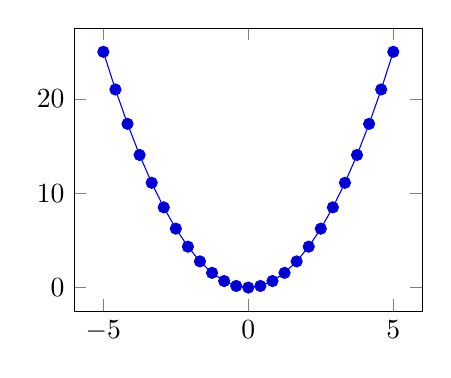
\begin{tikzpicture}\begin{axis}[width=6cm]\addplot{x^2};\end{axis}\end{tikzpicture}
\section{Two} More text here, \SI{3}{\metre}.
\end{document}
